\documentclass[12pt]{article}
\usepackage[papersize={7in,9in}, top=1in,bottom=1in,right=.65in,left=.65in]{geometry}
\usepackage{tpreamble}
\usepackage{newtxtext}  % Times text + CM-like math

\fancyfoot[C]{\textit{Combinatorics, \today, C. Castillo}} 

\begin{document}
	
	\title{Combinatorics}
	\author{Connor Castillo}
	\date{\today}
	\maketitle
	\tableofcontents
	
	\newpage
	\section{Counting Methods}
	\subsection{Counting Principles}
	\begin{theorem}[Addition Principle]
	Let $A_1, A_2, \dots, A_n$ be pairwise disjoint finite sets, so that
	\[
	A_i \cap A_j = \varnothing \quad \text{for } i \neq j.
	\]
	Then
	\begin{equation}
	\left| \bigcup_{i=1}^n A_i \right|
	= \sum_{i=1}^n |A_i|.
	\end{equation}
\end{theorem}
\begin{proof}
	Since the sets $A_1, \dots, A_n$ are pairwise disjoint, each element of
	\(\bigcup_{i=1}^n A_i\) belongs to exactly one of the sets $A_i$.
	Thus no element is counted more than once when summing their cardinalities.
	Therefore,
	\[
	\left| \bigcup_{i=1}^n A_i \right|
	= |A_1| + |A_2| + \cdots + |A_n|.
	\]
\end{proof}
	If the sets $A_1, \dots, A_n$ are not pairwise disjoint, the formula
$\left|\bigcup_i A_i\right| = \sum_i |A_i|$ can fail because overlapping
elements would be counted twice. However, modification to the principle via compensation of the over-count corrects such issues:
\begin{equation*}
	|A|+|B| - |A\cap B|
\end{equation*}
\begin{theorem}[Multiplication Principle]
	Let an experiment consist of $k$ stages, where stage $i$ admits $n_i$ possible
	outcomes for each outcome of the previous stages. Then the total number of
	possible outcomes of the experiment is
	\[
	n_1 n_2 \cdots n_k.
	\]
\end{theorem}


\begin{proof}
	Let $S_i$ denote the finite set of possible outcomes at stage $i$.
	An outcome of the experiment is determined by choosing one element from each
	$S_i$, so the sample space is the Cartesian product
	\[
	S = S_1 \times S_2 \times \cdots \times S_k.
	\]
	By the definition of Cartesian product,
	\[
	|S| = |S_1|\,|S_2|\cdots|S_k| = n_1 n_2 \cdots n_k.
	\]
\end{proof}

In general we may depict the multiplication principle through a choice tree that grows exponentially.
\begin{figure}[H]
	\centering
	\begin{tikzpicture}[
		grow=right,
		scale=0.7,
		transform shape,
		level distance=4.2cm,   % <-- THIS is what makes it span the page
		sibling distance=1.3cm,
		edge from parent/.style={draw, thick},
		every node/.style={font=\small},
		anchor=west
		]
		
		\node {Start}
		child { node {$a_1^{(1)}$}
			child { node {$a_2^{(1)}$}
				child { node {$a_3^{(1)}$}
					child { node {$\vdots$} }
					child { node {$a_k^{(1)}$} }
				}
				child { node {$\vdots$} }
				child { node {$a_3^{(n_3)}$} }
			}
			child { node {$\vdots$} }
			child { node {$a_2^{(n_2)}$} }
		}
		child { node {$\vdots$} }
		child { node {$a_1^{(n_1)}$} };
		
	\end{tikzpicture}
	
	\caption{The Choice Tree}
\end{figure}
	\subsection{Permutations}
	Consider a set $\set{1,2,...,n}$ of $n$ distinct elements. Then we define a \textit{permutation} of $\set{1,2,...,n}$ as a bijection 
\[
	f: \set{1,2,...,n}\to \set{1,2,...,n}
\]
\begin{definition}
	The \textbf{symmetric group} $S_n$ is a set containing all such permutations of a set $\set{1,2,...,n}$.
\end{definition}
	In cycle notation we commonly see permutations of $S_n$ as (12),(23), etc. For our purposes, we'll each element will appear as an ordered list. That is,
	\begin{equation*}
		f(1)f(2)f(3)f(4) = (12) 
	\end{equation*}
	where $f(1) = 2$, $f(2)=1$, and $f(3)=3,f(4)=4$.
\begin{proposition}
	Let $S_n$ denote the set of all permutations of the set $\set{1,2,...,n}$. Then
	\begin{equation*}
		|S_n| =  n!
	\end{equation*}
\end{proposition}
\begin{proof}
	By definition, a permutation is a bijection
	\[
		f: \set{1,2,...,n}\to \set{1,2,...,n}
	\]
	We construct a bijection by specifying the values of $f(1),f(2),...,f(n)$ sequentially. There are $n$ possible choices for $f(1)$. Once $f(1)$ is chosen, by way of injectivity, any subsequent selection must have $n-k$ possible choices for $f(k+1)$, and for the final selection of $f(n)$ there exists exactly one element to choose from. Then, by the multiplication rule, the total number of such sequences of choices is 
	\begin{equation*}
		n\cdot(n-1)\cdot(n-2)\cdots = n!
	\end{equation*}
	Thus, $|S_n| = n!$.
\end{proof}
\begin{eg}
	Take a triangle $D_n$ does though, with 3 distinct vertices, each labeled 1,2,3 respectively. The symmetric group $S_3$ of all permutations of the triangle will have $3!$ total permutations.
	\begin{center}
		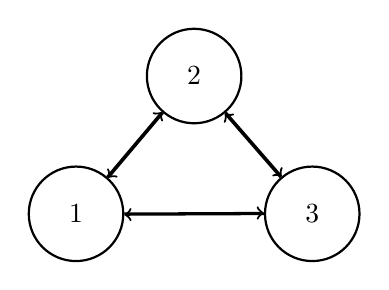
\begin{tikzpicture}[scale=.5,
			every node/.style={circle, draw, thick, minimum size=1.2cm},
			arrow/.style={->, thick}
			]
			
			% Nodes
			\node (1) at (0,0) {1};
			\node (3) at (6,0) {3};
			\node (2) at (3,3.5) {2};
			
			% Between 1 and 2
			\draw[arrow] ([xshift=-2pt,yshift=2pt]1) -- ([xshift=-2pt,yshift=2pt]2);
			\draw[arrow] ([xshift=2pt,yshift=-2pt]2) -- ([xshift=2pt,yshift=-2pt]1);
			
			% Between 2 and 3
			\draw[arrow] ([xshift=2pt,yshift=2pt]2) -- ([xshift=2pt,yshift=2pt]3);
			\draw[arrow] ([xshift=-2pt,yshift=-2pt]3) -- ([xshift=-2pt,yshift=-2pt]2);
			
			% Between 1 and 3
			\draw[arrow] ([yshift=3pt]1) -- ([yshift=3pt]3);
			\draw[arrow] ([yshift=-3pt]3) -- ([yshift=-3pt]1);
		\end{tikzpicture}
	\end{center}
\end{eg}
\begin{eg}
	Take a 52 card deck with no jokers. Shuffle the deck randomly. The total number of possible permutations of the deck is exactly 52!. 
\end{eg}
Up to this point, we have considered permutations of all $n$ elements.
We now ask how many permutations can be formed using only $k$ of the $n$
distinct elements. Rather than permuting all $n$ distinct elements, we may instead consider
permutations that involve only $k$ elements of the set.
\begin{definition}[Partial Permutation]
	The number of ways to choose and order $k$ elements from $n$ is 
	\begin{equation}
		P(n,k) = \frac{n!}{(n-k)!}
	\end{equation}
\end{definition}
\begin{eg}
	Consider a race of 10 total individuals. Determine the possible outcomes for the top 3 finishers. By the multiplication principle, we have $10\cdot 9\cdot 8$ selections for 3 stages, so we can write it as 
	\begin{equation*}
		\frac{10!}{(10-3)!} = \frac{(10)(9)(8)(7)\cdots(1)}{(7)\cdots(1)} = (10)(9)(8)
	\end{equation*}
\end{eg}

	\subsection{Combinations}
		Previously, for permutations we specifically cared about the ordering of the selections and distinguished them that way. Now, we look at the case for when we \textit{do not} consider the order. We derive the formula for \( \binom{n}{k} \) by separating the notions of
\emph{order} and \emph{choice}.\marginnote{Key idea: count something \emph{with} order, then divide the order out.} Return to the original partial permutation formulation
\begin{equation*}
	P(n,k) = \frac{n!}{(n-k)!}
\end{equation*}

Each unordered \( k \)-element subset is counted once for every permutation of
its elements. Since a set of \( k \) elements has \( k! \) orderings, we divide by \( k! \) to
correct for overcounting/collapse all orderings to one count.
\begin{definition}
	For integers \( n,k \) with \( 0 \le k \le n \), the \textbf{binomial coefficient}
	\[
	\binom{n}{k}
	\]
	is defined by \marginnote{Another useful way to interpret combinations is as the \emph{cardinality} of the collection of all $k$-element subsets of a given set.
	}
	\[
	\binom{n}{k} := \frac{n!}{k!(n-k)!}.
	\]
\end{definition}
\begin{eg}\label{eg1}
	Consider the set $\set{A,B,C}$ and suppose we want to choose 2 letters, where order does not matter. The ordered selections of 2 distinct letters will look like:
	\begin{align*}
		(A,B)&,(B,A) \\
		(A,C)&,(C,A)\\
		(B,C)&,(C,B) 
	\end{align*}
	There are exactly 6 pairs. Notice that for each selection of 2 letters we have $2!$ permutations. Now using $2!$ to collapse ordered pairs to a subset \begin{marginfigure}[-20mm]
		
		\begin{center}
			\includegraphics[scale=.3]{BCE}
			\caption{Illustration of Example \ref{eg1}. (1) being initial selection. (2) being results after permutations decided. (3) After collapsing redundancies.}
		\end{center}
		
	\end{marginfigure}
	\begin{align*}
		(A,B)&,(B,A) \to \set{A,B} \\
		(A,C)&,(C,A) \to \set{A,C}\\
		(B,C)&,(C,B) \to \set{B,C}
	\end{align*}
	so only 3 distinct subsets remain.
\end{eg}

\begin{theorem}[Identities]
	Binomial coefficients satisfy the following identities, 
	\begin{enumerate}[label=\roman*)]
		\item $\binom{n}{k} = \binom{n}{n-k}$
		\item $\binom{n}{k} = \binom{n-1}{k}+ \binom{n-1}{k-1}$
		\item $\binom{n}{0}+\binom{n}{1}+\cdots+\binom{n}{n-1}+\binom{n}{n} = 2^n$
	\end{enumerate}
\end{theorem}
\begin{proof}
	~ \marginnote{Note that part (iii) can be viewed as a count of all subsets of all sizes. Take $X = \set{1,2}$ for example. Each binomial coefficient corresponds as the following
	\begin{align*}
		\binom{2}{0} &\to \es \\
		\binom{2}{1} &\to \set{1},\set{2} \\
		\binom{2}{2} &\to \set{1,2}
	\end{align*}}[-20mm]
	\begin{enumerate}[label=\roman*)]
		\item
		Let $S$ be a set with $|S| = n$. Choosing a subset of $S$ with $k$ elements is equivalent
		to choosing which $n-k$ elements are excluded. Hence there is a bijection between
		$k$-element subsets and $(n-k)$-element subsets of $S$, so
		\[
		\binom{n}{k} = \binom{n}{n-k}.
		\]
		
		\item
		Let $S$ be a set with $|S| = n$ and fix an element $x \in S$.
		Every $k$-element subset of $S$ either contains $x$ or does not contain $x$.
		If it does not contain $x$, the $k$ elements are chosen from the remaining $n-1$
		elements, giving $\binom{n-1}{k}$ possibilities.
		If it does contain $x$, the remaining $k-1$ elements are chosen from the remaining
		$n-1$ elements, giving $\binom{n-1}{k-1}$ possibilities.
		Since these two cases are disjoint and exhaustive, we obtain
		\[
		\binom{n}{k} = \binom{n-1}{k} + \binom{n-1}{k-1}.
		\]
		
		\item
		Let $S$ be a set with $|S| = n$. The number of subsets of $S$ with exactly $k$ elements
		is $\binom{n}{k}$. Summing over all possible values of $k$ counts all subsets of $S$:
		\[
		\sum_{k=0}^n \binom{n}{k}.
		\]
		Alternatively, each element of $S$ may be either included or excluded from a subset,
		giving $2$ choices per element and hence $2^n$ subsets in total.
		Therefore,
		\[
		\binom{n}{0}+\binom{n}{1}+\cdots+\binom{n}{n} = 2^n.
		\]
	\end{enumerate}
\end{proof}
	\subsection{Inclusion and Exclusion Principles}
	Earlier, in section 1 we discussed counting principles under the assumption that sets were explicitly disjoint. Such conditions created scenarios for which \textit{over-counting} wasn't possible.
\begin{theorem}[Inclusion-Exclusion Principle]
	Let $A_1,\dots, A_n$ be finite sets. Then 
	\begin{equation}
		\bigg | \bigcup^{n}_{i=1}A_i \bigg |  = \sum^{n}_{i=1}|A_i| - \sum_{1\leq i \leq j \leq n}|A_i \cap A_j| + \cdots + (-1)^{n-1}|A_1\cap \dots \cap A_n|
	\end{equation}
\end{theorem}

\begin{figure}[h!]
	\begin{center}
		\includegraphics[scale=.6]{IEP}
		\caption{The Inclusion-Exclusion Principle}
		\label{Figure:IEP}
	\end{center}
\end{figure}
\begin{remark}
	The Inclusion Exclusion Principle is applicable to both permutations and combinations.
\end{remark}

The proof will be left up to exercise. Visually we may represent the principle with a small family first.


\newpage

In Figure \ref{Figure:IEP}, all points in each $A_i$ are first counted once. So we add all to the count individually as $|A_i|$. Now consider the double intersections. The points in each intersection (RGB) are counted again. So we have to remove them through double intersections $|A_i\cap A_j|$. However, during that process we also removed the points in the triple intersection (purple) completely ("uncounted three times"). Thus, we compensate by adding $|A_1\cap A_2\cap A_3|$. In the end, we have an accurate count.


\begin{eg}
	Consider the number of integers from 1 to 100 are divisible by 2 or 3. Let
	\begin{equation*}
		A = \set{n:2| n}, \quad B = \set{n: 3| n}
	\end{equation*}
	Then we have that $|A| = 50$, $|B| = 33$ and $|A \cap B| =16$. The final count is 67.
\end{eg}
\begin{eg}
		How many functions
		\[
		f:\{1,2,3,4\}\to\{a,b,c\}
		\]
		are surjective?	There are $3^4$ total functions.  
		For each $x\in\{a,b,c\}$, let
		\[
		A_x=\{\text{functions that omit } x\}.
		\]
		
		Then
		\[
		|A_x|=2^4
		\quad\text{and}\quad
		|A_x\cap A_y|=1^4
		\quad (x\neq y).
		\]
		
		By the Inclusion--Exclusion Principle,
		\[
		\begin{aligned}
			\text{Number of surjections}
			&=3^4-\binom{3}{1}2^4+\binom{3}{2}1^4 \\
			&=81-48+3 \\
			&=36.
		\end{aligned}
		\]	
\end{eg}




\end{document}
